% A lemma from Berkeley Math Tournament 2024
\begin{center}
    \textbf{\Huge A lemma from Berkeley Math Tournament 2024}
    \textbf{\large Solution by Azzam L. H.}
\end{center}

\section{Soal} 
The incircle of scalene triangle $\triangle{ABC}$ is tangent to $\overline{BC}, \overline{AC},$ and $\overline{AB}$ at points $D, E,$ and $F,$ respectively. The line $EF$ intersects line $BC$ at $P$ and line $AD$ at $Q.$ The circumcircle of $\triangle{AEF}$ intersects line $AP$ again at point $R \neq A$. If $I$ is the incenter of $\triangle{ABC}$, prove that $I,Q,R$ are collinear.


\newpage
\section{Solusi 1} 

    Misalkan $I$ adalah titik pusat lingkaran dalam $\triangle ABC$. Lalu, misalkan $H$ adalah perpotongan $AI$ dengan $FE$ dan $G$ adalah titik di $AD$ sehingga $IG \perp AD$.


    % --------

    \begin{center}
    \definecolor{rvwvcq}{rgb}{0.08235294117647059,0.396078431372549,0.7529411764705882}
    \definecolor{wewdxt}{rgb}{0.43137254901960786,0.42745098039215684,0.45098039215686275}
    \definecolor{ffqqtt}{rgb}{1.,0.,0.2}
    \definecolor{qqwwzz}{rgb}{0.,0.4,0.6}
    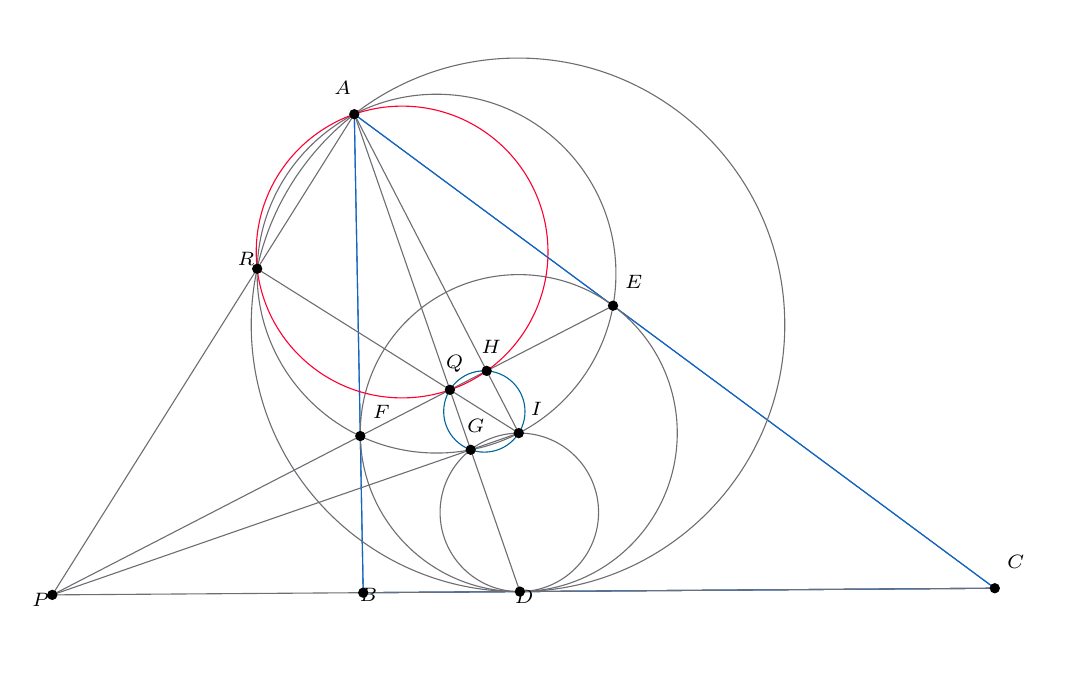
\begin{tikzpicture}[line cap=round,line join=round,scale=2.195]
    \clip(-2.5262,-2.7322) rectangle (3.3966,0.8768);
    \draw [color=rvwvcq] (-0.63636,0.37624) -- (-0.58477,-2.39231) -- (3.06937,-2.36652) -- cycle;
    \draw [color=rvwvcq] (-0.63636,0.37624) -- (-0.58477,-2.39231);
    \draw [color=rvwvcq] (-0.58477,-2.39231) -- (3.06937,-2.36652);
    \draw [color=rvwvcq] (3.06937,-2.36652) -- (-0.63636,0.37624);
    \draw [color=wewdxt] (-0.16058,-0.54634) circle (1.0380362210796263cm);
    \draw [color=wewdxt] (-0.63636,0.37624) -- (-2.38370,-2.40501);
    \draw [color=wewdxt] (-0.63636,0.37624) -- (0.32167,-2.38591);
    \draw [color=wewdxt] (-1.19823,-0.51810) -- (0.31520,-1.46892);
    \draw [color=wewdxt] (0.31520,-1.46892) -- (-2.38370,-2.40501);
    \draw [color=wewdxt] (0.31078,-0.84247) circle (1.543480381680652cm);
    \draw [color=wewdxt] (0.31844,-1.92742) circle (0.45850953677537326cm);
    \draw [color=wewdxt] (0.31520,-1.46892) circle (0.9170190735507474cm);
    \draw [color=wewdxt] (-0.63636,0.37624) -- (0.31520,-1.46892);
    \draw [color=wewdxt] (-2.38370,-2.40501) -- (3.06937,-2.36652);
    \draw [color=wewdxt] (0.86075,-0.73183) -- (-2.38370,-2.40501);
    \draw [color=ffqqtt] (-0.35978,-0.42119) circle (0.8440367068531726cm);
    \draw [color=qqwwzz] (0.11600,-1.34377) circle (0.23524616228583445cm);
    \begin{scriptsize}
    \fill (-0.6363594864428966,0.37624011380478484) circle (0.85pt);
    \fill (-0.5847715561111524,-2.3923131347934885) circle (0.85pt);
    \fill (3.0693735090540706,-2.366519160427666) circle (0.85pt);
    \fill (0.31520059641043696,-1.4689184684892247) circle (0.85pt);
    \fill (0.32167351327140564,-2.3859146967274776) circle (0.85pt);
    \fill (0.8607494049801038,-0.7318292752947456) circle (0.85pt);
    \fill (-0.6016593201398317,-1.486002808666865) circle (0.85pt);
    \fill (-2.383697782803491,-2.4050114420992523) circle (0.85pt);
    \fill (-0.08319198977616798,-1.2186258901885467) circle (0.85pt);
    \fill (-1.1982313596457344,-0.5180955879989007) circle (0.85pt);
    \fill (0.037078210261320965,-1.5653831644121856) circle (0.85pt);
    \fill (0.12954504242013595,-1.108916041980805) circle (0.85pt);
    \node[above left] at (-0.6090863018896259,0.4470246040774467) {$A$};
    \node[below] at (-0.5545070521035885,-2.322873310504881) {$B$};
    \node[above right] at (3.0954802773376593,-2.295583675878454) {$C$};
    \node[above right] at (0.3392281631427731,-1.4154929591761873) {$I$};
    \node[below] at (0.3460505693660278,-2.3296957191614878) {$D$};
    \node[above right] at (0.8850206610031466,-0.6786728242626617) {$E$};
    \node[above right] at (-0.5749742707733525,-1.4291377764894007) {$F$};
    \node[below left] at (-2.355622295042821,-2.3501629451313075) {$P$};
    \node[above] at (-0.05647139780599767,-1.1630638388817387) {$Q$};
    \node[left] at (-1.1685236121965086,-0.4603557472512468) {$R$};
    \node[above] at (0.06633191421258637,-1.5110066803686815) {$G$};
    \node[above] at (0.15502319511489707,-1.0539053003760313) {$H$};
    \end{scriptsize}
    \end{tikzpicture}
    \end{center}


    % --------
    Perhatikan bahwa $\dangle AFI = \dangle AEI = 90^\circ$ sehingga $A,F,I,E$ konsiklis dengan $AI$ sebagai diameternya. 
    Selanjutnya, karena $\dangle DGI = 90^\circ$ maka $D,G,I$ konsiklis dengan $DI$ sebagai diameternya. Di lain sisi, karena $\dangle IGA = 90^\circ = \dangle IFA$, maka $A,I,F,G$ konsiklis. 
    Lebih jauh, garis $IG$ merupakan \textit{radical axis} dari lingkaran $(AFGI)$ dan $(EGI)$.
    
    Selanjutnya, karena $DI \perp BC$ maka $(D,G,I)$ menyinggung $BC$ di $D$. Namun, karena $(DEF)$ juga menyinggung $BC$ di $D$ maka $BC$ merupakan \textit{radical axis} dari $(DEF)$ dan $(DGI)$.

    Di lain pihak, kita juga punya $EF$ merupakan \textit{radical axis} dari $(AEF)$ dan $(DEF)$.

    Perhatikan bahwa ketiga \textit{radical axis} $EF, BC, IG$ konkuren di suatu \textit{radical point}. Dari definisi di soal, karena $P$ adalah perpotongan $EF$ dan $BC$, maka didapat $P$ merupakan \textit{radical center} dari $(AEF), (DEF), (DGI)$.

    Misalkan $\Gamma$ adalah lingkaran yang melalui $A$ dan menyinggung $BC$ di $D$. Dari \textit{power of a point}, kita punya
    \begin{align*}
        PR \cdot PA = PF \cdot PE = PG \cdot PI = PD^2,
    \end{align*}
    sehingga didapat $R$ berada di $\Gamma$.

    Sekarang, jelas bahwa $EF \perp AI$ sehingga $\dangle QHI = 90^\circ = \dangle QGI$ yang menunjukkan $Q,H,I,G$ konsiklis. Oleh karena itu, dari \textit{power of a point} kita punya
    \begin{align*}
        PR \cdot PA = PG \cdot PI = PQ \cdot PH,
    \end{align*}
    sehingga didapat $A,R,Q,H$ konsiklis dengan $\dangle QRA = \dangle QHA = 90^\circ$. 
    Padahal kita juga tahu bahwa $A,R,F,I,E$ konsiklis dengan $AI$ sebagai diameternya yang langsung menyebabkan $\dangle IRA = 90^\circ$. Dari sini didapat $I,Q,R$ segaris. Terbukti.

\section{Solusi 2}
    Kita akan memakai konfigurasi gambar dari solusi 1. Observasi inversi terhadap lingkaran $(DEF)$. 
    Karena $\triangle IFH \sim \triangle IAF$ maka $IH \cdot IA = IF^2$ dengan $IF$ adalah jari-jari lingkaran $(DEF)$, maka $EF$ dipetakan ke $(AEF)$.
    Lalu, $\triangle IGD \sim \triangle IDP$ sehingga $IG \cdot IP = ID^2$ dengan $ID$ adalah jari-jari lingkaran $(DEF)$, maka $G$ dipetakan ke $P$.

    Perhatikan bahwa $AD$ adalah \textit{polar} dari \textit{pole} $P$ karena $IG \perp AD$.
    Misalkan $Q$ dipetakan ke $R'$ yang berada di $(AEF)$. Ingat bahwa $AI$ adalah diameter $(AEF)$ maka $IR' \perp AR'$. 
    Lalu, $AR'$ adalah \textit{polar} dari \textit{pole} $Q$. 
    Namun, perlu diingat bahwa karena $Q$ berada di \textit{polar} dari $P$, maka dari \textit{La Hire's theorem} didapat $P$ berada di \textit{polar} dari $Q$. Dari sini didapat $P$ berada di $AR'$.

    Dikarenakan $R$ dan $R'$ berada di $(AEF)$ serta $A,R,R',P$ segaris, maka didapat $R=R'$. Terbukti bahwa $I,Q,R'=R$ segaris.




